\section{Ausblick}

\begin{frame}{CP-Verletzung}
    \begin{columns}[T]
        \begin{column}{.6\textwidth}
            \begin{itemize}
                \item CPT-Theorem: Zeitumkehrsymmetrie sehr eng mit Asymmetrie von Materie und Antimaterie (CP) verknüpft
                \item Ein Blick in unser Universum
                \begin{itemize}
                    \item (fast) ausschlie\ss{}lich Materie und keine Antimaterie
                \end{itemize}
                \item Standard Modell der Kosmologie
                \begin{itemize}
                    \item Beim Urknall wurden exakt gleiche Mengen von Materie und Antimaterie produziert
                \end{itemize}
            \end{itemize}
            \centering
            \textbf{Wo ist die Antimaterie?}
        \end{column}
        \begin{column}{.4\textwidth}
            \centering
            
\includegraphics[height=.7\textheight]{img/ams02.png}\\
            \scalebox{.4}{(\textbf{Logo:} AMS-02, NASA/JSC)}
        \end{column}
    \end{columns}
\end{frame}

\begin{frame}{CP-Verletzung}
    \begin{columns}[T]
        \begin{column}{.6\textwidth}
            \textbf{Wo ist die Antimaterie?}
            \begin{itemize}
                \item<1-> da wir sie im Universum nicht finden, muss sie bereits zerfallen sein!
                \item<1-> \textbf{CP-Verletzung!}
                \item<1-> ... nur wo?
                \item<2-> Standard-Modell der Teilchenphysik (SM)
                \begin{itemize}
                    \item<2-> beste bestätigste Theorie für 3/4 fundamentalen Wechselwirkungen (Gravitation nicht enthalten)
                    \item<2-> enthält einen Sektor mit CP-Verletzung
                \end{itemize}
            \end{itemize}
        \end{column}
        \begin{column}{.4\textwidth}
            \centering
            \only<2>{%
            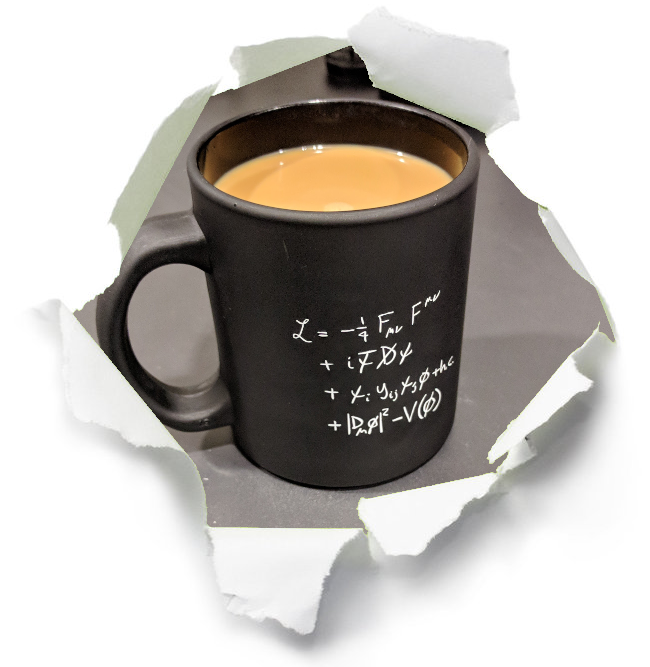
\includegraphics[height=.7\textheight]{img/cup.png}}
        \end{column}
    \end{columns}
\end{frame}

\begin{frame}{CP-Verletzung}
    \begin{columns}[T]
        \begin{column}{.6\textwidth}
            \textbf{CP-Verletzung - das Problem}
            \begin{itemize}
                \item CP-Verletzung ist im SM um \textbf{viele Größenordnungen zu klein} um die Asymmetrie im Universum erklären zu können
                \item Dennoch: bis heute \textbf{einzige} Erklärung für CP-Verletzung
                \item ... ist die Theorie richtig?
                \begin{itemize}
                    \item keine (signifikanten) Abweichungen bis zu erreichbaren Energien bekannt
                    \item vermutlich falsch für sehr große Energien (keiner weiß genau was in diesem Kontext \enquote{groß} bedeutet)
                \end{itemize}
            \end{itemize}
        \end{column}
        \begin{column}{.4\textwidth}
            \centering
            \begin{overpic}[height=.7\textheight]{img/cup.png}
            \end{overpic}
        \end{column}
    \end{columns}
\end{frame}

\begin{frame}{CP-Verletzung}
    \begin{columns}[T]
        \begin{column}{.5\textwidth}
            \textbf{CP-Verletzung - ein Lösungsansatz}
            \begin{itemize}
                \item Präzisionsmessungen
                \begin{itemize}
                    \item Vorhersagen vom SM werden verbessert
                    \item finden wir Abweichungen / Hinweise auf \textit{neue Physik?}
                \end{itemize}
                \item \textbf{LHCb}-Experiment (CERN)
                \begin{itemize}
                    \item Detektor am LHC-Speicherring
                \end{itemize}
            \end{itemize}
        \end{column}
        \begin{column}{.5\textwidth}
            \centering
            \begin{overpic}[width=\textwidth]{img/lhcb_collaboration.png}
            \end{overpic}
        \end{column}
    \end{columns}
\end{frame}

\begin{frame}{Das LHCb-Experiment}
    \enquote{LHCb is an experiment set up to explore what happened after the Big Bang that allowed matter to survive and build the Universe we inhabit today}\\
    {\footnotesize (\texttt{http://lhcb-public.web.cern.ch})}

    \begin{columns}[T]
        \begin{column}{.7\textwidth}
            \begin{itemize}
                \item ... bis jetzt (leider?) noch keine signifikante Abweichung vom SM gefunden
                \item Die Suche geht weiter - es bleibt spannend!
            \end{itemize}

            \vspace{5mm}
            \begin{center}
                Vielen Dank für Ihre Aufmerksamkeit!
            \end{center}
        \end{column}
        \begin{column}{.3\textwidth}
            \centering
            \begin{overpic}[height=.7\textheight]{img/lhcb_pit.png}
            \end{overpic}
        \end{column}
    \end{columns}
\end{frame}
